\documentclass[10pt]{article}
\usepackage{blindtext}
\usepackage{graphicx}
\usepackage{float}
\usepackage{wrapfig}
\usepackage{multicol}
\usepackage{color}
\usepackage[utf8]{inputenc}
\usepackage[T2A]{fontenc}
\usepackage{fancybox,fancyhdr}
\usepackage{lastpage}
\usepackage{amsmath}
\usepackage[warn]{mathtext}
\usepackage{listings}
\usepackage{color}
\usepackage{longtable}

\usepackage{geometry}
\geometry{
	a4paper,
	top=74pt,
	bottom=40pt,
	left=40pt,
	right=40pt,
}

\lstset{
	language=C++,
	tabsize=2,
	basicstyle=\footnotesize\ttfamily,
  breaklines=true,
  keepspaces=false,
  showspaces=false,
  showstringspaces=false, 
}
\fancyhf{}
\fancyhead[L]{Nizhny Novgorod State University: Presskachat (Burdukov, Kulandin, Sukharev)}
\fancyhead[R]{Page~\thepage~of~\pageref{LastPage}}

\setlength{\columnseprule}{0.5pt}
\def\columnseprulecolor{\color{black}}

\renewcommand\contentsname{Содержание}
\renewcommand{\headrulewidth}{2pt}

\begin{document}
\pagestyle{fancy}

\begin{multicols}{2}

\tableofcontents

\section{Setup}
\subsection{Instructions}
\begin{enumerate}
  \item Открыть VSCode
  \item Настроить сборку, отладку, запуск
  \begin{itemize}
    \item Debug: g++ -std=c++17 -Wall 
    -Wextra -Wno-unused-result -pg 
    -DLOCAL -O0 -fsanitize=address 
    -fsanitize=undefined 
    -fstack-protector-strong -fstack-check 
    -fno-sanitize-recover=all -o main.exe main.cpp
    \item Release: g++ -Wall -Wextra 
    -Wno-unused-result -O2 -DHOME=1 -o main.exe main.cpp
  \end{itemize}  
  \item touch template.cpp makefolders.sh
  \item Набрать шаблон и makefolders
  \item ./makefolders
\end{enumerate}
\subsection{Template}
\lstinputlisting{template.cpp}
\subsection{Make folders}
\lstinputlisting[language=bash]{run.sh}
\subsection{Stress}
\lstinputlisting[language=bash]{stress.sh}
\subsection{Фишечки}
\lstinputlisting[language=bash]{Algorithms/fishki.cpp}
\section{Algorithms}
\subsection{Pragmas}
\lstinputlisting{Algorithms/pragmas.cpp}
\subsection{PBDS}
\lstinputlisting{Algorithms/PBDS.cpp}
\subsection{Sieve $O(N)$}
\lstinputlisting{Algorithms/strong_sieve.cpp}
\subsection{2D geometry + Сonvex hull}
\lstinputlisting{Algorithms/geoma.cpp}
\subsection{GCDEX + Диофантово уравнение}
\lstinputlisting{Algorithms/gcdex.cpp}
\subsection{Strong comp + bridges $O(N)$}
\lstinputlisting{Algorithms/Graphs/strong_components _and_bridges.cpp}
\subsection{Cutpoints $O(N)$}
\lstinputlisting{Algorithms/Graphs/cutpoints.cpp}
\subsection{Max flow Dinic $O(N^2M)$}
\lstinputlisting{Algorithms/Graphs/Flows/Dinic.cpp}
\subsection{Min Cost Max Flow $O(N^2M^2)$}
\lstinputlisting{Algorithms/Graphs/Flows/MCMF.cpp}
\subsection{HLD $O(N\log{N})$}
\lstinputlisting{Algorithms/Graphs/HLD.cpp}
\subsection{LCA $O(N\log{N})$}
\lstinputlisting{Algorithms/Graphs/LCA.cpp}
\subsection{Sparse table $O(N\log{N})$}
\lstinputlisting{Algorithms/sparse_table.cpp}
\subsection{Fenwick $O(N\log{N})$}
\lstinputlisting{Algorithms/fenwick.cpp}
\subsection{Сartesian tree $O(N\log{N})$}
\lstinputlisting{Algorithms/cartesian_tree.cpp}
\subsection{BigInt $O(N^2)$}
\lstinputlisting{Algorithms/BigInt.cpp}
\subsection{Prefix function $O(N)$}
\lstinputlisting{Algorithms/Strings/kmp.cpp}
\subsection{Z function $O(N)$}
\lstinputlisting{Algorithms/Strings/z.cpp}
\subsection{Manacher $O(N)$}
\lstinputlisting{Algorithms/Strings/manacher.cpp}
\subsection{Suffix array $O(N\log{N})$ + LCP $O(N)$}
\lstinputlisting{Algorithms/Strings/suf_mas.cpp}
\subsection{Персистентное ДО $O(N\log{N})$}
\lstinputlisting{Algorithms/Persistent ST/1.cpp}
\subsection{FFT $O(N\log{N})$}
\lstinputlisting{Algorithms/FFT.cpp}
\subsection{Simplex method}
\lstinputlisting{Algorithms/simplex.cpp}
\subsection{2-SAT $O(N\log{N})$}
\lstinputlisting{Algorithms/2sat.cpp}
\end{multicols}
\newpage
\section{Формулы}
\begin{itemize}
\item Всего \textbf{генераторов} (пораждающих элементов) в группе по модулю N -- $\varphi(\varphi(N))$
\item Генератор существует только у чисел $2, 4, p^a, p^{2a}$
\item \textbf{Длина группы генератора} -- $\varphi(N)$
\item \textbf{Теорема Эйлера}: $a^{\varphi(N)} \equiv 1 \pmod{N}$, где gcd$(a, b) = 1$
\item \textbf{Малая теорема Ферма}: $a^{p-1} \equiv 1 \pmod{p}$, где gcd$(a, p) = 1$ и p - простое
\item \textbf{Порядком} r называется наименьшее положительное такое, что $x^r \equiv 1 \pmod{N}$.
По теореме Лагранжа r будет делителем $\varphi(N)$. Поэтому, чтобы найти порядок нужно перебрать все делители $\varphi(N)$
\item \textbf{Число цифр в периоде дроби} $\frac{a}{b}$ равно m : $(10^{m}*a - a) \mod{b} = 0$. $b = 2^x*5^y*B$ -- длина предпериода равна $max(x, y)$
\item \textbf{Китайская теорема об остатках}
\\ Дано: 
\begin{equation*}
  \begin{split}
    &c\mod a = a_1 \\
    &c\mod b = b_1 \\
    &c\mod (a * b) = ?
  \end{split}
  \end{equation*}
\\ Решение:
\begin{equation*}
  \begin{split}
    &a*x + b*y = 1 (gcdex)\\
    &c = (a_1 + a * x * (b_1 - a_1)) \mod (a * b)
  \end{split}
  \end{equation*}
\item \textbf{Числа стирлинга 2-го рода}
\begin{equation}
  \begin{split}
    &S_2(n, k) = 
    \left\{
    \begin{array}{cc}
    S_2(n-1, k-1) + k \cdot S_2(n-1, k), & 0 < k \le n\\
    0, & n = 0\\
    1, & k = n
    \end{array}
    \right.\\
    &S_2(n, k) = \frac{1}{k!}\sum\limits_{i=0}^k(-1)^{i}\binom{k}{i}(k - i)^n\\
    &S_2(n + 1, m + 1) = \sum\limits_{k=0}^n\binom{n}{m} \cdot S_2(k, m)\\
    &\sum\limits_{k=0}^nS_2(n, k) = B_n \text{ -- число Белла}
  \end{split}
\end{equation}
\begin{longtable}[c]{lllllllllll}

n\textbackslash{}k & 0 & 1 & 2 & 3 & 4 & 5 & 6 & 7 & 8 & 9
\\
0 & 1 & & & & & & & & &
\\
1 & 0 & 1 & & & & & & & &
\\
2 & 0 & 1 & 1 & & & & & & &
\\
3 & 0 & 1 & 3 & 1 & & & & & &
\\
4 & 0 & 1 & 7 & 6 & 1 & & & & &
\\
5 & 0 & 1 & 15 & 25 & 10 & 1 & & & &
\\
6 & 0 & 1 & 31 & 90 & 65 & 15 & 1 & & &
\\
7 & 0 & 1 & 63 & 301 & 350 & 140 & 21 & 1 & &
\\
8 & 0 & 1 & 127 & 966 & 1701 & 1050 & 266 & 28 & 1 &
\\
9 & 0 & 1 & 255 & 3025 & 7770 & 6951 & 2646 & 462 & 36 & 1
\\

\end{longtable}
\item \textbf{Числа стирлинга 1-го рода}
\begin{equation}
  \begin{split}
    &S_1(n, k) = 
    \left\{
    \begin{array}{cc}
    S_1(n-1, k-1) + (n - 1) \cdot S_1(n-1, k), & 0 < k \le n\\
    0, & n = 0\\
    1, & k = n
    \end{array}
    \right.\\
    &S_1(n + 1, m + 1) = \sum\limits_{k = 1}^n S_1(n, k) \cdot \binom{k}{m} = n! \cdot \sum\limits_{k=0}^n\frac{S_1(k, m)}{k!}\\
    &S_1(n, m) = \sum\limits_{k=1}^n S_1(n + 1, k + 1) \cdot \binom{k}{m} \cdot (-1)^{m - k}\\
    &S_1(n + m + 1, m) = \sum\limits_{k=0}^m (n + k) \cdot S_1(n + k, k)
  \end{split}
\end{equation}
\begin{longtable}[c]{llllllll}

n\textbackslash{}k & 0 & 1 & 2 & 3 & 4 & 5 & 6
\\

0 & 1 & & & & & &
\\
1 & 0 & 1 & & & & &
\\
2 & 0 & 1 & 1 & & & &
\\
3 & 0 & 2 & 3 & 1 & & &
\\
4 & 0 & 6 & 11 & 6 & 1 & &
\\
5 & 0 & 24 & 50 & 35 & 10 & 1 &
\\
6 & 0 & 120 & 274 & 225 & 85 & 15 & 1
\\

\end{longtable}
\item \textbf{Числа Белла} (кол-во различных способов разбиения множества): 0:1, 1:1, 2:2, 3:5, 4:15, 5:52, 6:203, 7:877, 8:4140, 9:21147, 10:115975\\
\begin{equation}
  \begin{split}
    &B_{n + 1} = \sum\limits_{k = 0}^n\binom{n}{k} \cdot B_k\\
    &B_{n + p} \equiv B_n + B_{n + 1}\pmod{p}, \text{ p - простое}\\
    &B_{n + p^m} \equiv m \cdot B_n + B_{n + 1}\pmod{p}, \text{ p - простое}
  \end{split}
\end{equation}

\item \textbf{Числа Каталана}: : 0:1, 1:1, 2:2, 3:5, 4:14, 5:42, 6:132, 7:429, 8:1430, 9:4862, 10:16796, 11:58786, 12:208012, 13:742900,
14:2674440, 15:9694845
\begin{equation}
  \begin{split}
    &С_{n} = \sum\limits_{i = 0}^{n - 1}C_i \cdot C_{n - 1 - i}\\
  \end{split}
\end{equation}
\item \textbf{Задача двух клик} переходит в двудольность дополнения исходного графа, для восстановления пишем рюкзак
\item \textbf{В неориентированном графе Эйлеров путь} существует, когда 
\begin{itemize}
  \item Степень каждой вершины четна
  \item Существует ровно две вершины нечетной степени, степени всех остальных четны
\end{itemize}
В первом случае каждый Эйлеров путь является Эйлеровым циклом
\item \textbf{В ориентированном графе Эйлеров путь} существует, когда все рёбра принадлежат одной компоненте сильной связности и
\begin{itemize}
  \item Полустепени захода и схода каждой вершины равны
  \item Существует одна вершина, для которой полустепень захода на единицу
  больше полустепени исхода, еще одна вершина, для которой полустепень исхода на единицу больше полустепени захода,
  а во всех остальных вершинах полустепени исхода и захода равны
\end{itemize}
\item \textbf{Максимальный поток} = минимальный разрез. Вершины принадлежащие минимальному разрезу находятся запуском dfs из истока по ребрам, у которых поток != 0
\item \textbf{Максимальное число реберно-непересекающихся путей} = макс поток (каждое ребро капасити = 1). Пути можно найти жадно из истока к стоку
\item \textbf{Вершинно-непересекающиеся пути} находятся макс потоком через расщепление вершины на две
\item \textbf{Теорема Холла}. Совершенное паросочетание существует, когда для $\forall X$:
$\left|X\right| \le \left|f(X) \right|$, где $X$ -- множество вершин левой доли, $f(X)$ -- множество соседей Х
\item \textbf{Теорема Кёнига. Минимальное вершинное покрытие} = максимальное паросочетание в двудольном графе. 
Вершины не принадлежащие минимальному вершинному покрытию, образуют 
\textbf{максимальное независимое множество}.\\
Алгоритм нахождения минимального вершинного покрытия:
\begin{enumerate}
  \item Находим максимальное паросочетание
  \item Ориентировуем ребра:
  \begin{itemize}
    \item Из паросочетания -- из правой доли в левую
    \item Не из паросочетания -- из левой в правую
  \end{itemize}
  \item Запускаем DFS из ненасыщенных парасочетанием вершин левой доли.
  \item Ответ: $\left|\text{непосещенные вершины левой доли}\right| + \left|\text{посещенные вершины правой доли}\right|$
\end{enumerate}
\item \textbf{Покрытия вершинно-непересекающимися путями (только в ацикличном ориентированном графе)}.
Строим двудольный граф с вершиной как в левой, так и в правой доле.
Соединяем ребром вершины из левой и правой долей, если они есть в исходном графе.
Количество путей = N - макс пар соч в двудольном графе
\item \textbf{Покрытие общими путями}.
Делаем граф из прошлого пункта + добавляем ребра $a->b$, такие, что
в исходном графе есть путь от а к b. Количество путей = N - макс пар соч в двудольном графе
\item \textbf{Матрица поворота вокруг любой заданной оси}.\\
Пусть ось вращения задана единичным вектором $\mathbf{v} = (x,y,z)$, а угол поворота $\theta$.
\begin{equation*}
  M(\mathbf{v}, \theta) = \left(
  \begin{array}{cccc}
  \cos{\theta} + (1 - \cos{\theta})x^2 & (1 - \cos{\theta})xy - (\sin{\theta})z & (1 - \cos{\theta})xz + (\sin{\theta})y\\
  (1 - \cos{\theta})yx + (\sin{\theta})z & \cos{\theta} + (1 - \cos{\theta})y^2 & (1 - \cos{\theta})yz - (\sin{\theta})x\\
  (1 - \cos{\theta})zx - (\sin{\theta})y & (1 - \cos{\theta})zy + (\sin{\theta})x & \cos{\theta} + (1 - \cos{\theta})z^2
  \end{array}
  \right)
\end{equation*}
\end{itemize}
\newpage
\begin{figure}[h]

  \centering
  
  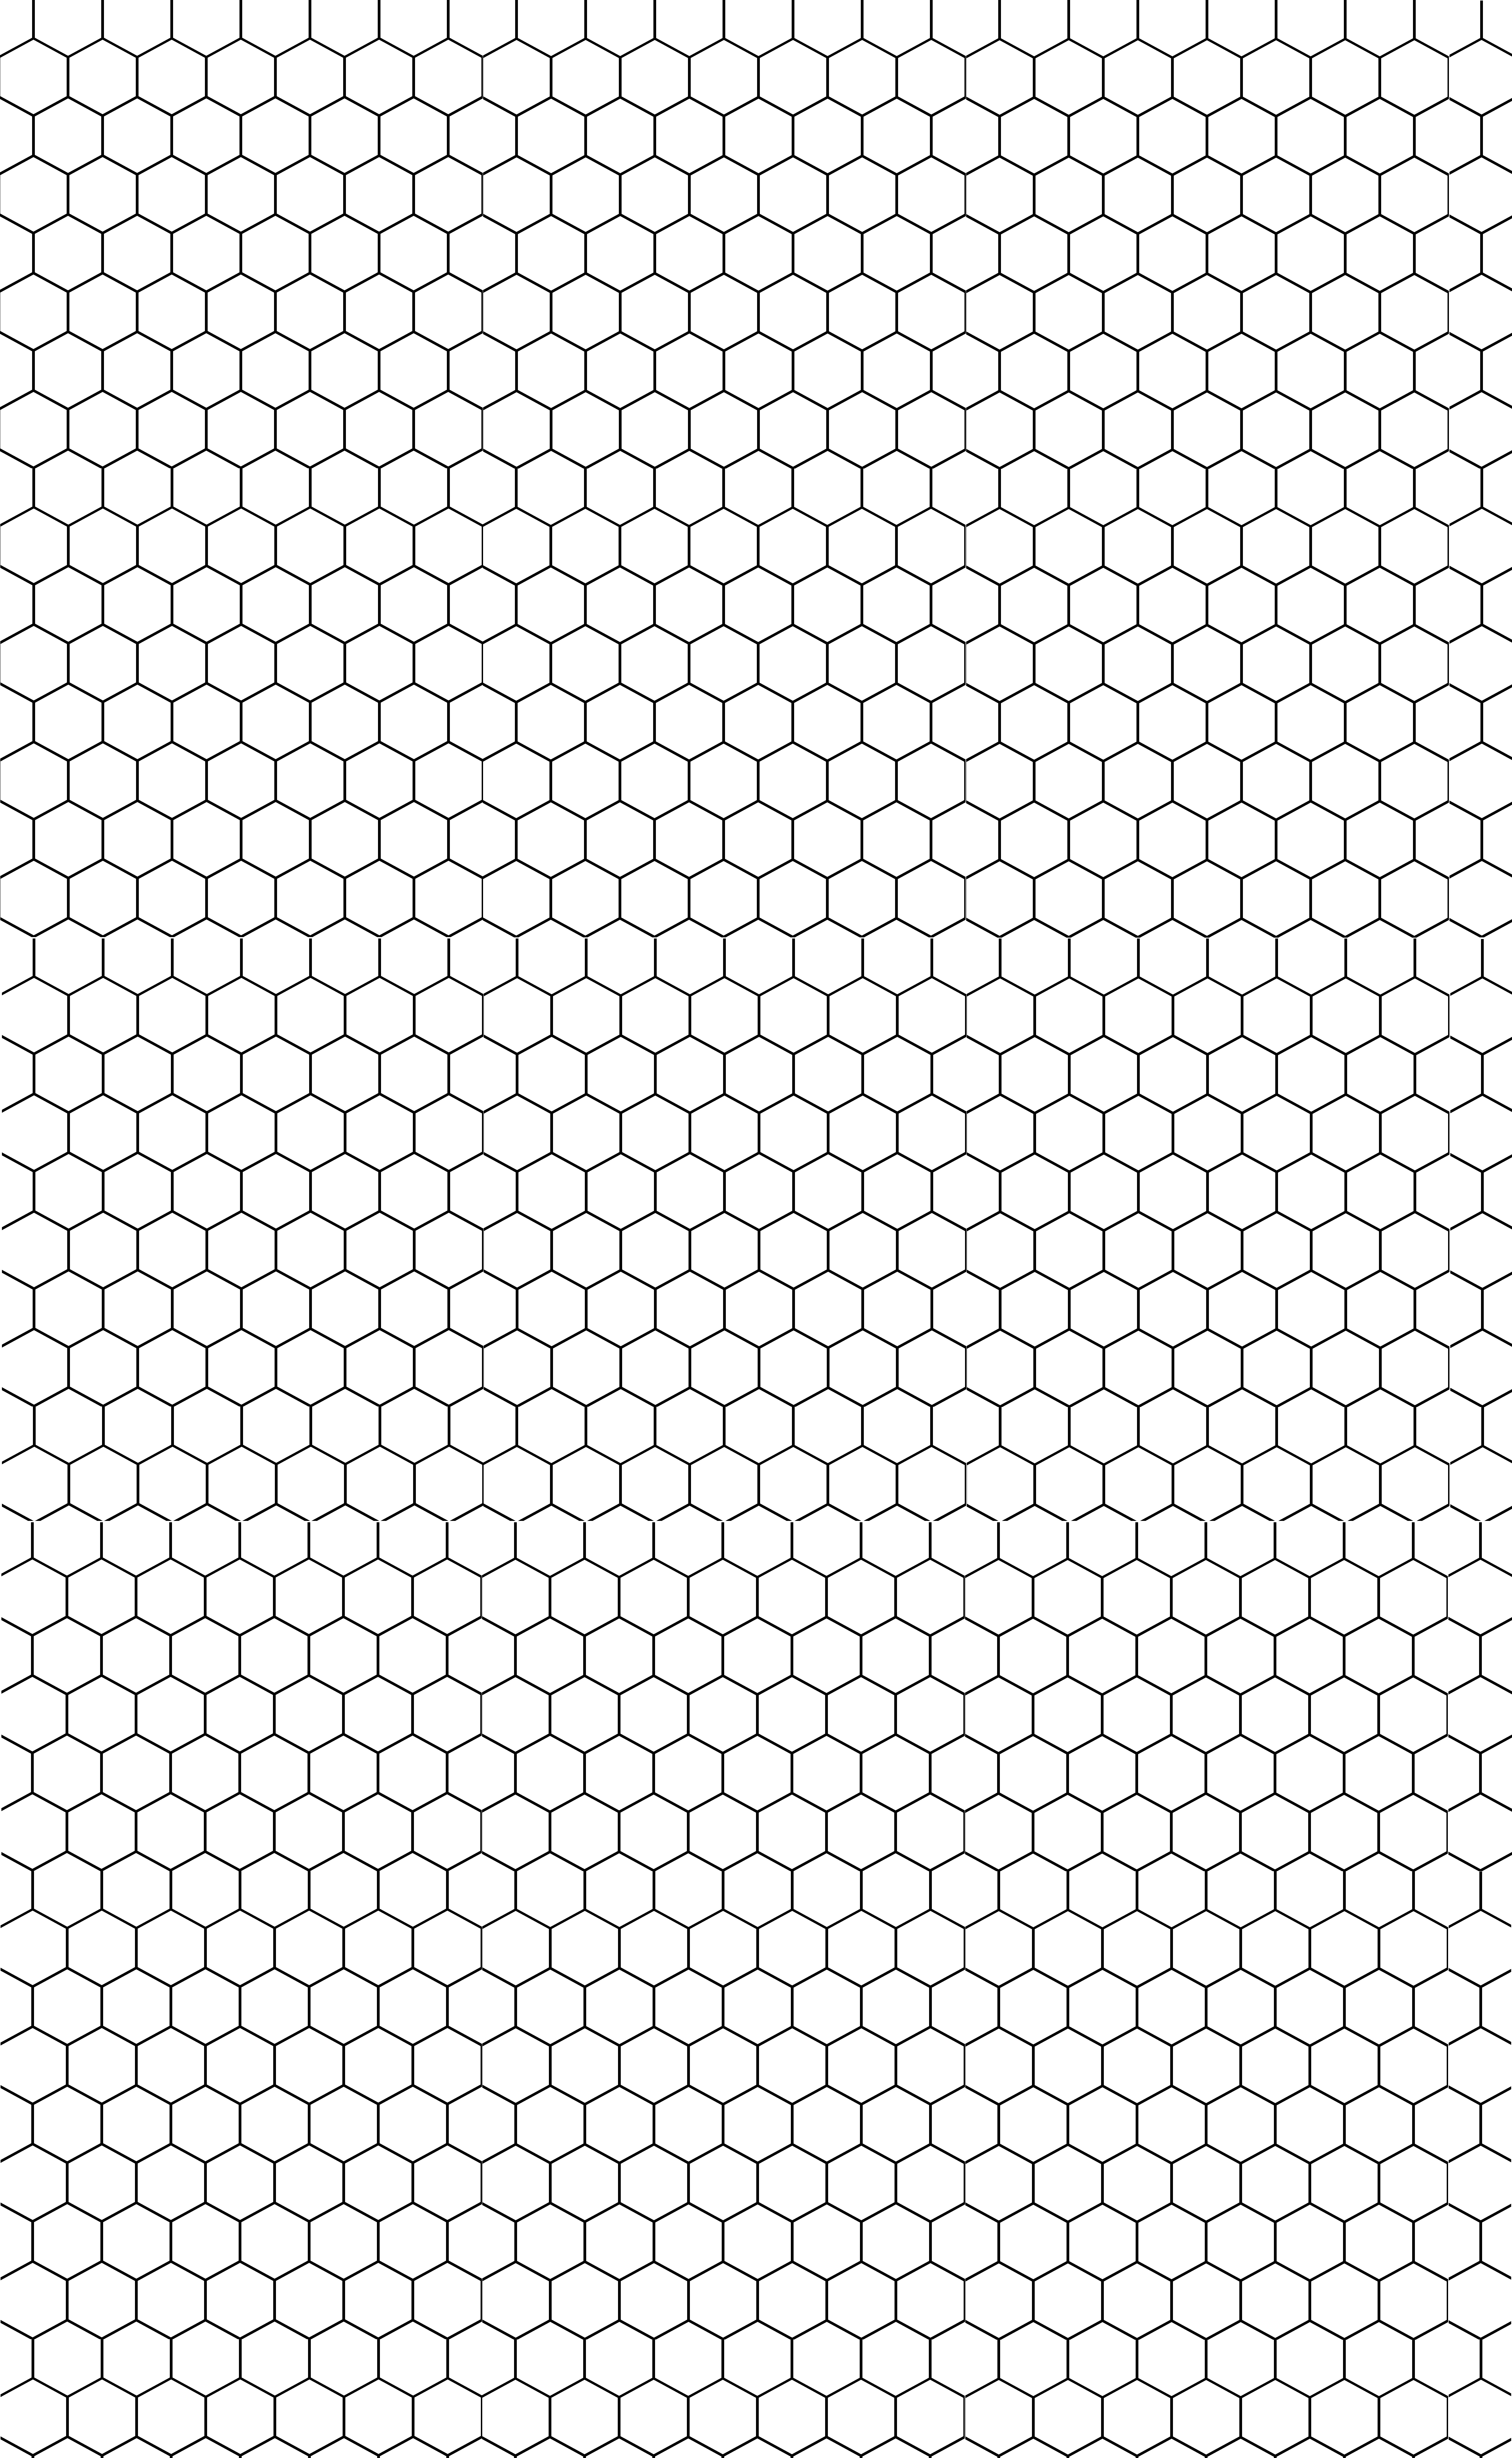
\includegraphics[width=0.8\linewidth]{hex.png}
  
  \label{fig:mpr}
  
  \end{figure}
\end{document}